\chapter{Specification}

	Based on the business requirements we decided that the back-end part of the application must take these five divisions into account: Customers, Employees, Vehicles, Orders and Notifications. In the rest of the chapter we are describing features that these modules should have.
	
	\section{Customers}
		Customers are uniquely identified by telephone number. We also want to store about each of them these information:
		\begin{itemize}
			\item ID
			\item Name
			\item Note
			\item Fraud status
		\end{itemize}
	
		With Customer entity we are able to do these operations:
		\begin{itemize}
			\item Create and confirm
			\item Update
			\item Destroy
			\item Recover password
			\item Login and logout
			\item List favourite locations
			\item List all customers and show specific customer
		\end{itemize}
		\subsection{Operation create and confirm}
			There are two ways how customer can be created. It is either directly through registration or indirectly by creating new order.
			
			Directly registered customers are created in exchange for telephone number, password and optional name. With this type of account customer can later login with provided password. Application must verify given telephone.
			
			Indirectly registered user is created during creation of new order for telephone number, which doesn't belong to any existing customer. This customer type is just envelop for the purpose of tracking information and statistics - mostly for better customer support. This account type can not be used for authentication. Indirectly registered user can be directly registered later without any difference to normal direct registration.
		
		
		\subsection{Operation update}
			Customer can update only it's own name and password. Employees are able to change any customer's name, note and fraud status.
		\subsection{Operation destroy}
			Destroy the customer can be invoked by that customer or the administrator. Orders made by that customer are not deleted - the order has no customer then.
		\subsection{Operation password recovery}
			In case of lost password is customer able to recover it. At first customer asks for the recovery with its telephone. In return it receives recovery token via SMS. This token is valid for 5 minutes. With this token and telephone number can new password be set. Customer is able to ask for token resend - which will invalidate last token, generate new token and sends it via SMS.
		\subsection{Operation login and logout}
			With login operation we receive login token in exchange for telephone number and password. We send this token with each request to be authenticated.
			Customer can login if and only if it is directly registered and confirmed.
			Logout just invalidates the session - customer must log in again to be authenticated.
		\subsection{Operation list favourite locations}
			Our application must provide list of customer favourite places. In the front-end part of the application should be this implemented in the part where customer chooses its pick-up and drop-off location. 
			
			Main priority is to provide list of these places fast = less than one second. Most important are first five returned places and the most likely places based on current conditions should be among them These places should be ordered with respect to the given location ( in reality current customer location or pick-up location when choosing drop-off ). It should also take into account whether customer chooses pick-up or drop-off. These recommendations should be based on customer's order history and respect start - finish relation of the orders. 
			
			Let's imagine customer that has two routes - it often goes from pub to its home and sometimes goes from its home to gym. Application then should return its home as first item when looking for drop-off recommendation from unknown pick-up place. Application should also return gym as first item when user is asking for drop-off recommendation with pick-up at home, even though pub is much more frequent place in its history.
			
			 Show the favourite locations list of a specific user is permitted only for that specific user or any employee.
		 
		\subsection{Operation list all customers and show specific customer}
			Our API must provide information of the customers created in our application.
			Show specific customer's data is available only for the customer itself or any employee. 
			
			List all the customers is available for administrator only, because the list of the customers is one of the most valuable asset of the taxi company and we don't want to provide it for the staff. Of course the employee could get all the customers by going one by one via operation show, but it takes more time so this is for our purpose enough.
		
	\section{Employees}
		There three types of employees - administrators, dispatchers and drivers. Employees unlike customers are identified via email. We store these information about each one:
		\begin{itemize}
			\item Email
			\item Name
			\item Photograph
		\end{itemize}
		
		In our application we also have information about the employees shifts - whether it is at work or not. For drivers we also process current locations and their order queues. 
		
		Operations on employees are almost the same as operations on customers. Operations differs mainly in permissions. 
		\begin{itemize}
			\item Create and confirm
			\item Update
			\item Destroy
			\item Recover password
			\item Login and logout
			\item List all employees and show specific employee
		\end{itemize}
		
		\subsection{Shifts}
		 Employees could be in three statuses: 
			\begin{itemize}
				\item available
				\item unavailable
				\item pause
			\end{itemize}
			Available means that the employee is on site and can handle orders. Unavailable is when it is not at work. Pause status is there for the situations when the employee knows that it won't be available for a while but wants to finish its orders.
			
			Switching directly from available to unavailable should be only in cases of emergency, e.g. driver has flat tire and cannot continue. Employees will be instructed not to do so for better customer experience. 
			
			Employee is available to list the history of its shifts and administrator is available to list shifts for all the employees. Changing shifts (available statuses) are employees allowed only for themselves.
		
		\subsection{Driver locations}
			Each driver from the shift start until the shift end sends at regular intervals its location. Driver's current location is able to set only driver itself. Get the last  driver's location is can anyone, so the front-end can display the current location of arriving driver even for anonymous customer. 
		
		\subsection{Driver order queues}
			Each driver has a queue of orders that are assigned to it. Administrator can see all the queues, driver can see only its own queue.
	
		\subsection{Operation create and confirm}
			Employee can be created by administrator only. In exchange for the email, optional name and image the confirmation email is sent to the employee. Then the employee is by clicking the link in email redirected to front-end page, where it fill its password. The link contains confirmation token which will the front-end together along with the optional name and image send to our application.
	
		\subsection{Operation update}		
		Employee can update its password, name and image. Administrator can besides these fields change also employee role.
		\subsection{Operation destroy}
		Only administrator can remove the employee from the application. When the employee is removed, all the shifts and driver queue is removed too. Orders associated with the employee remains in system but the corresponding employee field is removed.
		\subsection{Operation recover password}
		Recovering the forgotten password is exactly the same as in the customers case - except the reset password token is sent via email in link to the front-end.
		\subsection{Operation login and logout}
		Only difference in these operations between the employees and customers is that the employees login with email instead of telephone number. Everything else is the same.
		\subsection{Operation list all employees and show specific employee}
		Show all the employees or specific employee can only administrators and dispatchers. The rest (drivers, customers, anonymous users) can see only drivers who are on shift.
		
		There is also different attributes which are shown for different people. Public attributes that anyone can see are id, name and image of the employee. Email, roles, and other attributes like timestamps of creation or update are available only to employee itself, dispatchers or administrators.
	
	\section{Vehicles}
		Taxi company has the vehicle fleet we want to have in our system too. Each driver's shift starts with selecting the vehicle driver will ride in, so the customer can see and choose the car that fit its needs.
		
		 For each vehicle we have these information:
		\begin{itemize}
			\item name
			\item internal vehicle number for taxi company used for communication
			\item plate
			\item image
			\item how many customers can fit in - required
			\item whether the vehicle is available for driving or not e.g. is temporarily in the car repair shop
		\end{itemize}
		These operations with vehicles our application supports:
		\begin{itemize}
			\item Create and update
			\item Show all and specific
			\item Destroy
		\end{itemize}
		\subsection{Operation create, update and destroy}
			Only administrators can create, update and destroy company's vehicles. They can manipulate all the specified information. When the car is deleted, all the corresponding shifts or orders will have set the null value instead of the vehicle.
		\subsection{Operation show all and specific vehicle}
			Administrators can see all the vehicles, others can see only the active ones. 
			
			Operations show to anyone all the attributes besides the internal vehicle number and the availability. Employees can see all of the attributes.
	\section{Orders}
	 	Order is key entity in this application. Each order must go through process from creation to successful finish or cancellation. 
	 	
	 	There are two types of orders. The first one we call scheduled - customer wants the taxi to arrive to its location at specific date and time. In this type of order arriving at the specified time is crucial. The other type is when customer just need taxi and sooner it arrives then better.
	 	
	 	Order can be come from two sources - dispatchers and customers directly.
	 	
	 	About each order we would like to have these information:
		
		\begin{itemize}
			\item id
			\item status 
			\item driver who takes care of it
			\item vehicle by which it is processed with
			\item pick-up and drop-off location coordinates and addresses
			\item passenger count
			\item note
			\item contact telephone in case the customer is ordering for someone else
			\item estimated price
			\item whether the assigned driver can not be changed (is explicitly chosen)
			\item VIP (just internal flag for the taxi company)
			\item flight number - in case that the order is to/from the airport
			\item customer
			\item assigned dispatcher
			\item date and time when the customer wants the taxi to arrive to the pick-up location (scheduled pick-up)
			\item source - whether it was created by dispatcher or directly by customer via front-end application
		\end{itemize}
		Also with order we want to know track these time parameters. In parenthesis are the terms how the times will be referenced in the whole thesis and application:
		\begin{itemize}
			\item created time
			\item application estimate when the driver starts arriving to customer (start est.)
			\item when the driver started arriving to customer (start)
			\item estimation when will the driver arrive to the customer (arrived time est.)
			\item actual time when driver arrived to the customer - (arrived time)
			\item estimation and actual time when the driver has picked up  customer and starts driving to the drop-off destination (picked-up time est., picked-up time)
			\item finish time estimation and actual finished time(finish time, finish time est.)
		\end{itemize}
	
		Our goal is to have as much data about the order as possible, so we can later make statistics and analysis based on them. 
		
		These actions are needed for the orders module:
		\begin{itemize}
			\item show all / specific order
			\item list driver arrivals
			\item create order
			\item defraud and process
			\item confirm by driver
			\item refuse by driver
			\item arriving
			\item change arrive time
			\item arrived
			\item customer not on its place
			\item picked up
			\item change drop off time or location
			\item finished
			\item fraud
			\item my orders for dispatcher
			\item cancel
		\end{itemize}
		
		Because the order process is very complex, we decided to sum it up in the one illustration. This scheme displays all the order statuses (green), actions that can be done with the order and this application implements them (violet), time parameters we track (blue) and notifications which are sent in these actions (blue).
		
		\begin{figure}[H]
			\centering
			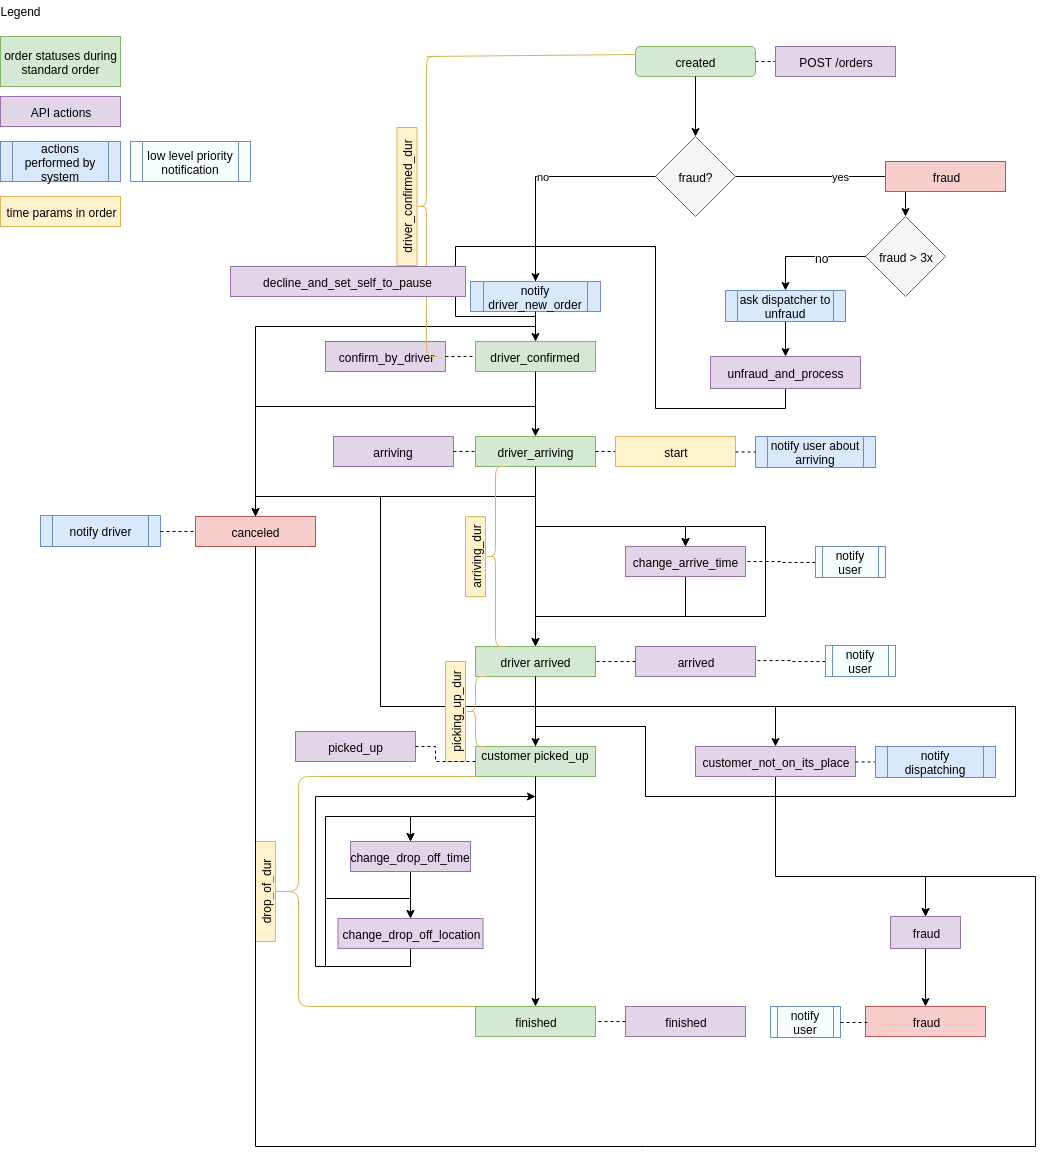
\includegraphics[width=\textwidth]{orders/order_process_scheme.png}
			\caption{Order process scheme}\label{order-process-scheme}
		\end{figure}
	
			In next subsections we describe in detail all the actions, their prerequisites, conditions and outputs.
		
		\subsection{show all / specific order}
			Employees can see all the orders, customers can see only orders which they have made (even via dispatcher).
			
			We show specific attributes to the specific user types. Anyone (e.g. anonymous customers) can see order status, created time, arrived time est., finish time est.,  driver and vehicle assigned to it. 
			
			Customer whose order it is can get also coordinates and address of start and finish, passenger count, note, contact telephone, estimated price, whether assigned driver is selected explicitly, VIP flag, flight number, arrived time, scheduled pick up and source.
			
			Employees can besides all of the attributes above  see assigned dispatcher and all the tracked times, estimations and original estimations.
			
			For showing all orders we also show total order count for the specified query.
			
			Orders support basic filtering. We can get orders which are created since and until as parameters. We can also get only scheduled orders. Orders can be filtered also based on their status - we can set multiple statuses we want to show.
			
			Orders are paginated - we can set via parameters which page to show and how much orders per page.
			
			
		\subsection{List driver arrivals}
		This action must return for the start and finish location list of the available drivers with their cars including the estimated arriving times to that location. This information then dispatcher tells the customer in case the order is via dispatching. In the other case customer can see it directly in its app.
		
		It also takes driver parameter for the case that the customer wants the specific driver and only checks for the arrival time.
		
		This list is provided for anyone - even anonymous users.
		
		In case there is no driver available for such conditions it should return no available drivers result.
		\subsection{Create order}
			Order can be created two ways. Either it is via dispatcher - customer calls the taxi company and the dispatcher will make the order. 
			
			If the customer is marked as fraud, new order is automatically marked as fraud one, thus it does not continue in process and the creator is informed about that. If the number of fraud orders in history for the customer is less than three, one of the dispatchers on shift get the notification whether this customer should be forgiven and order processed. If the user has more than three fraud orders, dispatchers won't even get the notification about defrauding.
			
			Both the customer and dispatcher can explicitly choose a driver who takes care of the order. 
			
			Order will be assigned to the driver who can be at the pick-up location earliest. Scheduled orders are meant to be assigned to drivers manually by dispatchers.
			
			 If no driver is available for the specified parameters, it must return error.
			 
			 After this action, order status is \textit{created}.
		\subsection{Defraud and process}
			This action is called by dispatcher as response to defraud notification - when it wants to forgive the customer frauds in history and wants to process that order.
			
			If the customer is forgiven, it is marked as non-fraud and order is normally processed. Customer is from that moment on considered as standard non-fraud user, so it can create subsequent orders without limitation. The forgiveness is though not definite - possible next fraud order will renew original customer's fraud order count and add one fraud more.
		\subsection{Confirm by driver}
			When order is assigned to driver, driver confirms via this action that it knows about it and is able to take it. Until then, the arrive time estimation is very rough. This action can be performed only by the assigned driver and only if the order status is \textit{created}.
			
			This action changes the order status to \textit{driver\_confirmed}
		\subsection{Refuse by driver}
			Driver also can refuse order. We suppose that this will happen only in emergency cases. If driver refuses order, it is removed from its queue and passed to the next available driver. If there's none, order is marked as cancelled.
			
			To refuse the order, its status must be \textit{created} and it can be done by driver assigned to the order only.
		\subsection{Arriving}
			Driver can have more confirmed orders in its queue. When it starts to go to the customer, it calls the Arriving endpoint. This change the order status to \textit{driver\_arriving} and recalculate the time of arrival to customer. In this moment it should very precise estimation - driver should be slowed down only by the traffic which is included in the Google Maps API. Thanks to that we send the SMS to the customer with the estimated arrive time in this moment.
			
			The order status must be for calling this action must be \textit{driver\_confirmed} and it can be called by driver assigned to order only. 
		\subsection{Change arrive time}
			Driver can correct the estimated arrive time based on its experience or unexpected complications during the journey.
			
			Correct the arrive time can only driver for his own orders which are in the \textit{arriving} state.
		\subsection{Arrived}
			This request is sent when driver arrives to the pick-up place. This changes order status to \textit{arrived} and updates following times estimations, because now we have precise moment of arrival.
			
			It can be set by the assigned driver only and only when the order status is \textit{arriving}.
		\subsection{Customer not on its place}
		In case that the driver can not get in touch with the customer this action is called. It sends the notification to the dispatching and the dispatching take care of the situation and communicate the problem between the driver and the customer. This can situation can be resolved only by the to ways. Either is customer found and picked up or it is not and the order is marked as fraud. 
		
		This action can be called only when the order status is \textit{arrived} and by the driver assigned to the order.
		\subsection{Picked up}
		In a point when the driver picks up the customer and is ready to ride to drop-off location is this request sent. Because now we know the picking up time precisely, drop off estimations can be recalculated. Also this action changes the order status to \textit{customer\_picked\_up}.
		
		This action can be called only when order status is \textit{arrived} and only by driver whose is the order.
		\subsection{Change drop off time or location}
			Customers often don't know what they want, so in our application driver assigned to the order can change in this point the drop off time and also the location. This change leads to the recalculation of the estimated times. 
		\subsection{Finished}
			Order is marked by driver as finished when he successfully handled whole order and is ready to go to another customer.
		\subsection{Fraud}
			Order can be marked as fraud from the \textit{driver\_arrived} and \textit{cancelled} order statuses. Mark order as fraud can only driver assigned to the order. Marking as fraud resets the customers fraud count back to all the fraud orders it has.
		\subsection{Cancel}
			Order can be cancelled by the driver assigned to order, dispatcher or the customer whose order it is. In case that the customer is anonymous it can be cancelled by anyone - because we can not distinguish separate anonymous users.
			
			Only valid order statuses from which can order be cancelled are \textit{'created'}, \textit{'driver\_confirmed'}, \textit{'driver\_arriving'} and \textit{'driver\_arrived'}.
			
		\subsection{My orders for dispatcher}
			Each order is assigned to some dispatcher. These dispatcher than take care of the customers and in case of the problems must be able to see that problem and handle it with the customer. For such purpose there is this endpoint. Dispatcher can see all its order with important details such as the actual time estimations, original estimations, customer number, assigned driver and so on.
			
			This endpoint shows only orders which are not finished, cancelled or fraud and the results are paginated.			
	
	\section{Notifications}
		Our system must have a way how to send messages to the users on specific actions. As described in orders section, there are three types of notifications:
		\begin{itemize}
			\item driver has new order
			\item customer is not at pick-up location
			\item new order from fraud customer
		\end{itemize}
		
		Each type contains specific data. Driver has new order contains the order id, customer not at pick-up location contains driver id and name, customer id and telephone. New order from fraud customer contains order and customer id.
		
		
		Notification system is passive = users call our \textit{list notifications} action in regular intervals. When user resolves notification, it can mark the notification as resolved.
		
		
		\subsection{Operation list notifications}
			This operation returns all the notifications for the current user. The list is paginated via \textit{page} and \textit{per\_page} parameters. It also supports filtering only unresolved notifications.
		\subsection{Operation mark as resolved}
			Notification can be marked as resolved only by the person to who it belongs. 